\documentclass{article}
\usepackage[hidelinks]{hyperref}
\usepackage{graphicx}
\usepackage{amsfonts}
\usepackage{amsmath}
\usepackage{enumitem}
\usepackage{polski}
\usepackage[utf8]{inputenc}
\usepackage{indentfirst}
\usepackage{float}
\title{Dokumentacja projektu dotyczącego optymalnego układania klocków na planszy}
\author{Abdelkarim Ahmed, Cacko Agata, Hernik Aleksandra}
\begin{document}
\maketitle
\section{Opis projektu}
\section{Opis algorytmu}
Wykorzystany algorytm jest algorytmem zachłannym z określoną parametrem liczbą nawrotów $k$. W każdym kroku algorytmu uruchamiane jest $k'$, gdzie $1 \le k' \le k$ (w sekcji wielowątkowość znajduje się wyjaśnienie, od czego jest uzależniona ich dokładna liczba). Każdemu wątkowi odpowiada jeden z $k$ najlepszych wyników uzyskanych w poprzednim kroku, gdzie najlepszy wynik to taki, dla którego wartość funkcji kosztu jest jak najmniejsza -- każdy z nich dla swoich danych wejściowych znajduje $k$ najlepszych rozwiązań. Znalezienie rozwiązań polega na sprawdzeniu dla każdego klocka każdego jego rotacji -- najpierw wybierana jest jego pozycja, a następnie liczony koszt całej planszy. $k$ rozwiązań takich, że funkcja kosztu obliczona na planszy z położonym danym klockiem w danej rotacji jest najmniejsza, to rozwiązanie dla danego wątku. Następnie, spośród ułożeń otrzymanych przez wszystkie wątki ($1 \le k' \le k$, zatem otrzymywane jest od $k$ do $k^2$ ułożeń) wybierane jest $k$ najlepszych. Ogólny schemat działania algorytmu podsumowuje poniższy diagram:
\begin{figure}[H]
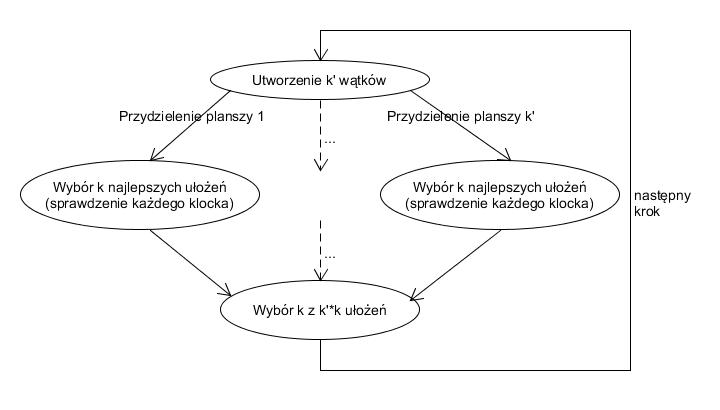
\includegraphics[width=\textwidth]{schemat_algorytmu.png}
\caption{Ogólny schemat działania algorytmu}
\end{figure}
\subsection{Wybór pozycji dla klocka}
\subsection{Funkcje kosztu planszy}
\subsection{Wielowątkowość}
\subsection{Łączenie wyników}
\subsection{Struktura danych}
\section{Testy}
%\subsection{zestaw pierwszy...}
%\subsection{zestaw drugi...}
\section{Wnioski} %z testów
\end{document}